\chapter{Results} \label{results}
%\begin{figure}[H]
%\centering
%    \begin{minipage}{0.45\textwidth}
%%        \centering
%        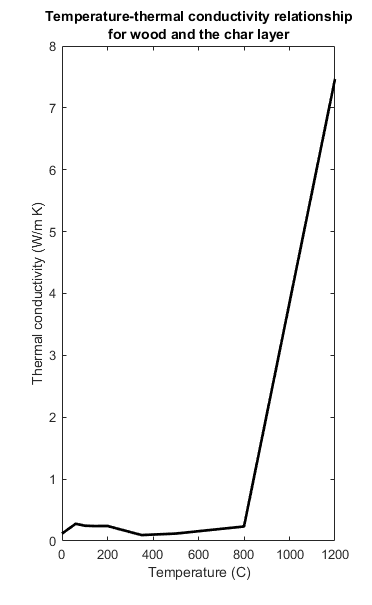
\includegraphics[width=0.9\textwidth]{figures/resultsk_cropped.png} % first figure itself
%        \caption{The resulting $\kappa$-values }
%        \label{kresult_fig}
%    \end{minipage}
%    \begin{minipage}{0.45\textwidth}
%%        \centering
%        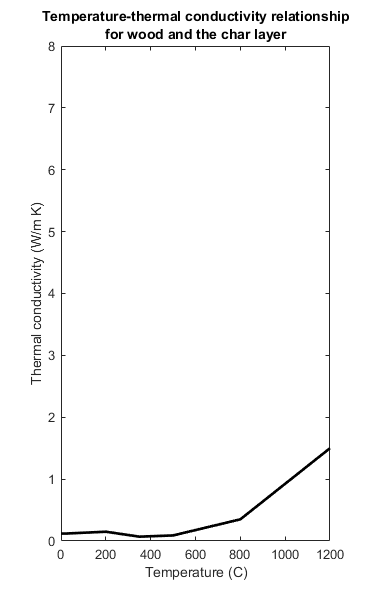
\includegraphics[width=0.9\textwidth]{figures/eurok_samescale_cropped.png} % second figure itself
%        \caption{The original $\kappa$-values}
%        \label{scalekeuro_fig}
%    \end{minipage}
%\end{figure}\

The results of running the algorithm until 20 000 acceptable values are found is shown below.

\begin{figure}[H]
	\label{kresult_euro_fig}
	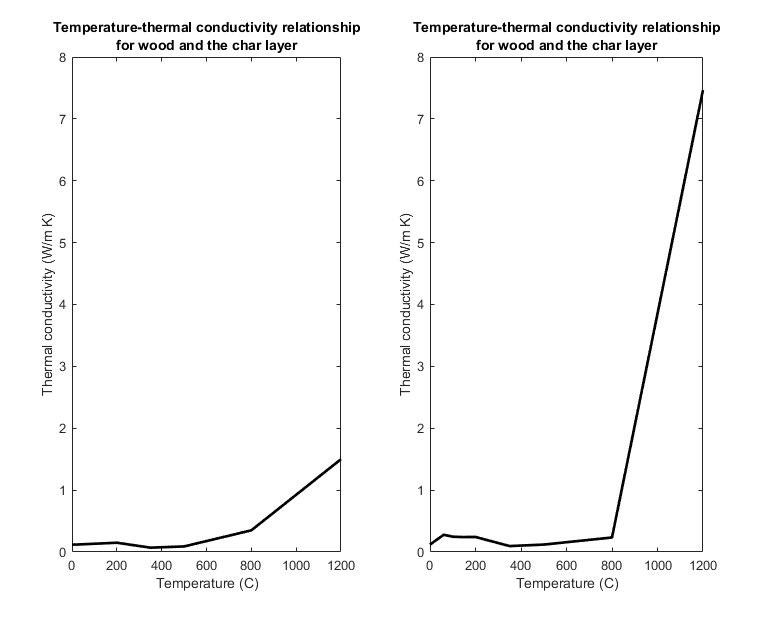
\includegraphics[width=\linewidth]{figures/euro_and_results.png}
\end{figure}
\begin{figure}[H]
	\label{og_modeldata}
	\centering
	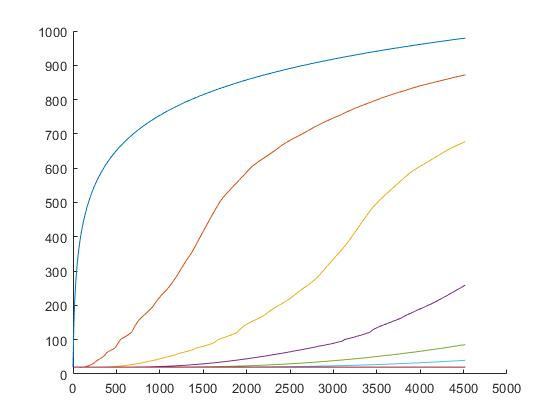
\includegraphics[width=5.5in,]{figures/originalmugraph.jpg}
	\caption{Output of finite element model using $\kappa$-values as indicated in EN 1995:1-2-2004}
\end{figure}

\begin{figure}[H]
	\label{data_newk}
	\centering
	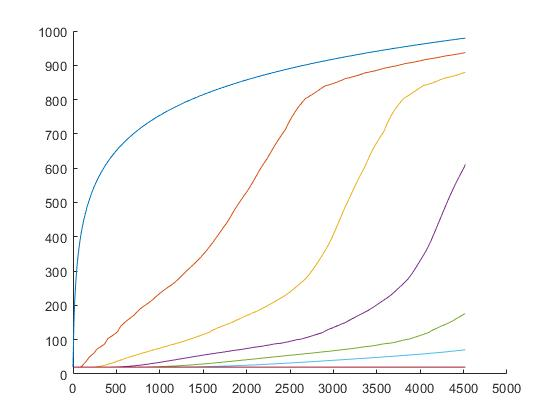
\includegraphics[width=5.5in,]{figures/rough_average_graph.jpg}
\end{figure}